\newpage
%
% Návrh
%
\ifthenelse {\boolean{bachelor}}
{
	%\section{Design}
	\section{Návrh}
}
{
	%\chapter{Design}
	\chapter{Návrh}
}
\label{section:design}

%
% Návrh uchovávania textov v databázach
%
\ifthenelse {\boolean{bachelor}}
{
	%\subsection{Subsection}
	\subsection{Návrh uchovávania textov v databázach}
}
{
	%\section{Subsection}
	\section{Návrh uchovávania textov v databázach}
}
\label{subsection:our_design_persisting_data}
Dáta budeme ukladať v dokumentovej databáze MongoDB. Keďže spracovávané dáta sa dajú rozdeliť do troch kategórií, budeme využívať primárne tri databázové kolekcie na ich ukladanie. Sú to:

\begin{my_itemize}
	\myitem sentences,
	\myitem rules,
	\myitem texts.
\end{my_itemize}
	
Pri návrhu sme vychádzali z princípu čo najjednoduchších kolekcií, ktoré budu obsahovať iba relevantné informácie.
V nasledujúcich častiach ich opíšeme bližšie aj s názornými ukážkami.

%
% Kolekcia texts
%
\ifthenelse {\boolean{bachelor}}
{
	%\subsection{Subsection}
	\subsubsection{Kolekcia texts}
}
{
	%\section{Subsection}
	\subsection{Kolekcia texts}
}
V kolekcií \textit{texts} sa ukladajú celé texty, ktoré sú spracovávané. 

Kolekcia obsahuje iba jedno pole textového typu slúžiace na uloženie textu v pôvodnom tvare. Štruktúra uložených dát v kolekcií \textit{texts} je zobrazená na obrázku~\fullref{fig:texts_collection_structure}.

\begin{figure}[H]
	\begin{center}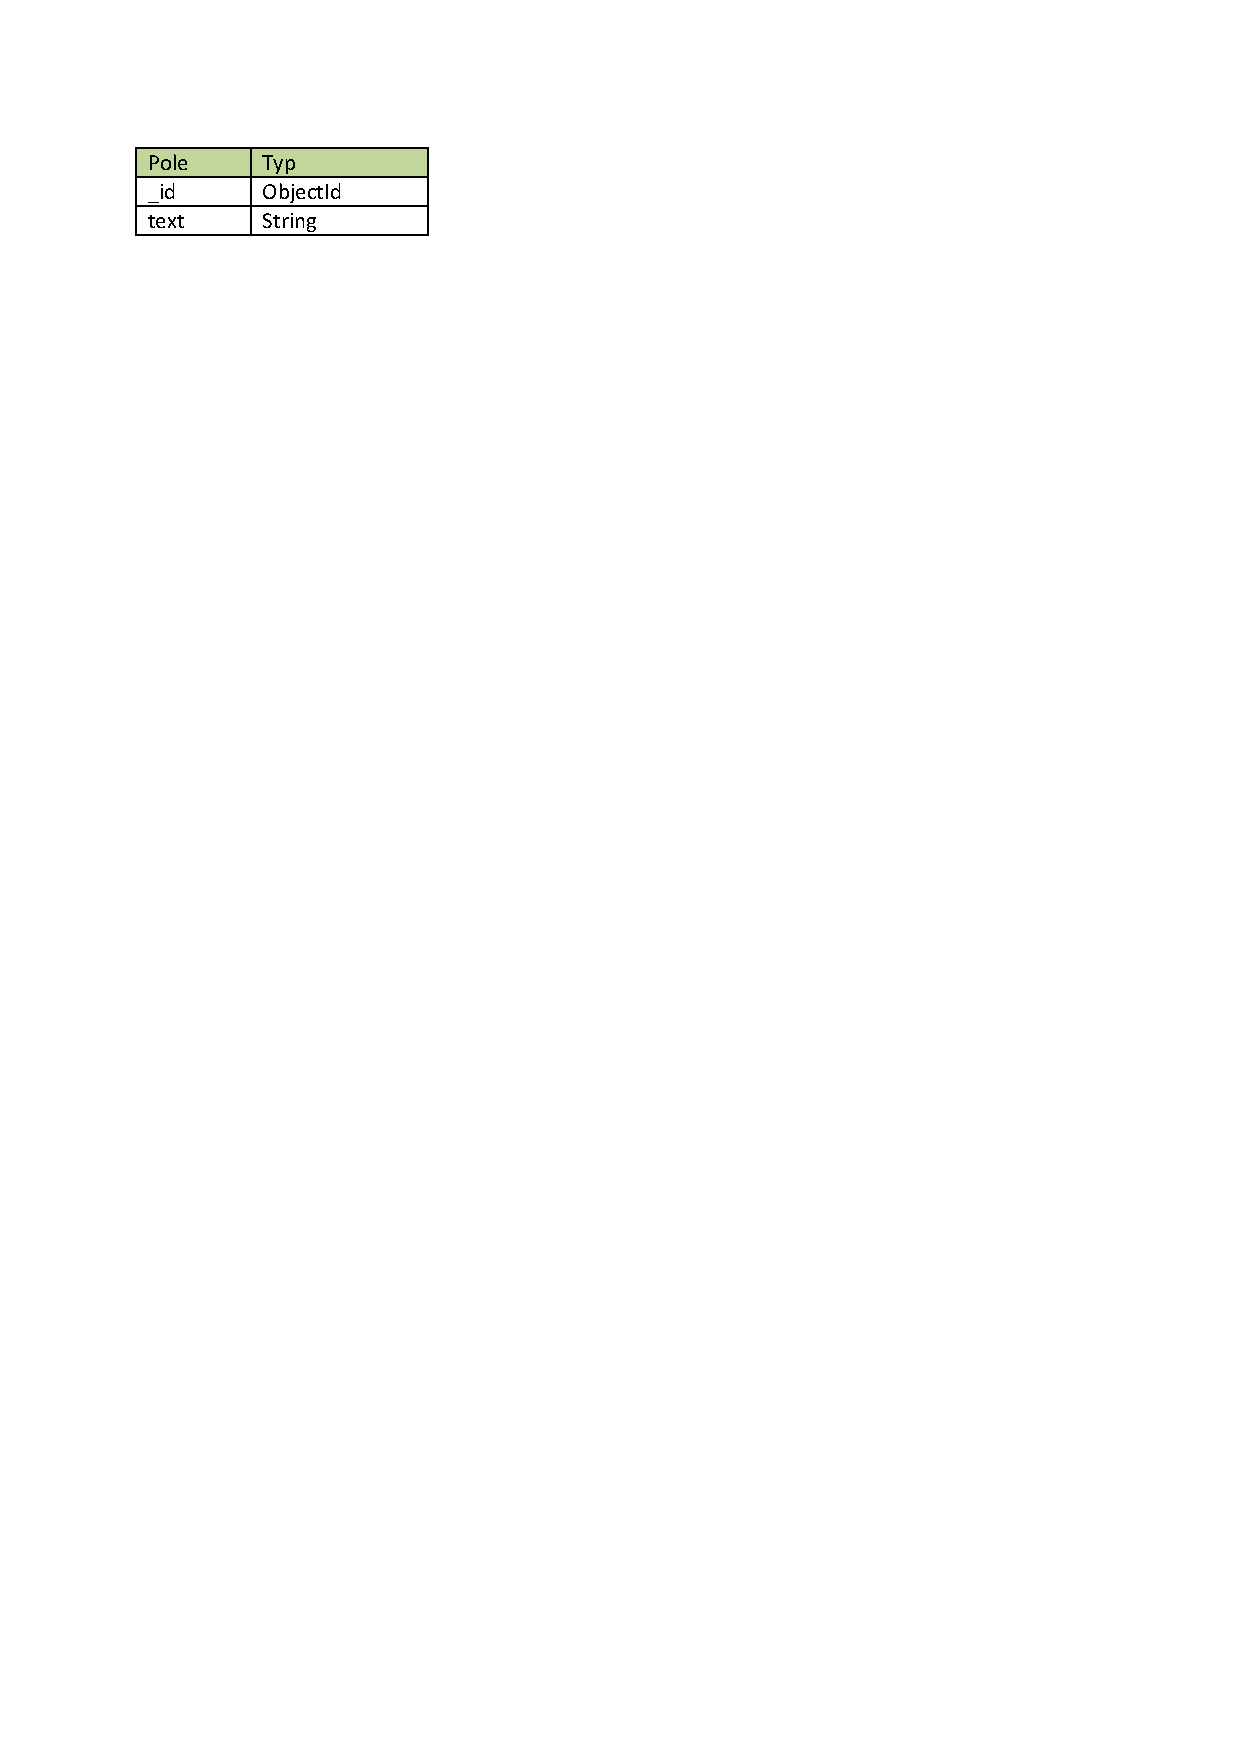
\includegraphics[scale=0.60]{texts_collection}\end{center}
	\caption[Štruktúra kolekcie texts]{Štruktúra kolekcie texts}\label{fig:texts_collection_structure}
\end{figure}

%
% Kolekcia sentences
%
\ifthenelse {\boolean{bachelor}}
{
	%\subsection{Subsection}
	\subsubsection{Kolekcia sentences}
}
{
	%\section{Subsection}
	\subsection{Kolekcia sentences}
}
V ďalšej kolekcii \textit{sentences} ukladáme spracovávané vety a vytvorené poznámky z týchto viet, pričom vety sa odkazujú na texty, z ktorých pochádzajú v kolekcií \textit{texts}. Umožní nám to jednoducho zistiť, v akom texte sa daná veta nachádzala.

Dáta sú uložené v dokumentoch, ktoré obsahujú tri polia. Jedno, textové, určené na uchovanie pôvodného znenia vety, druhé tiež textové na uchovanie novo vytvorenej vety po spracovaní vety uloženej v prvom poli a tretie pole, ktoré bude odkazovať na záznam v kolekcii \textit{texts}. Štruktúra dát v tejto kolekcií je načrtnutá na obrázku~\fullref{fig:sentences_collection_structure}.

\begin{figure}[H]
	\begin{center}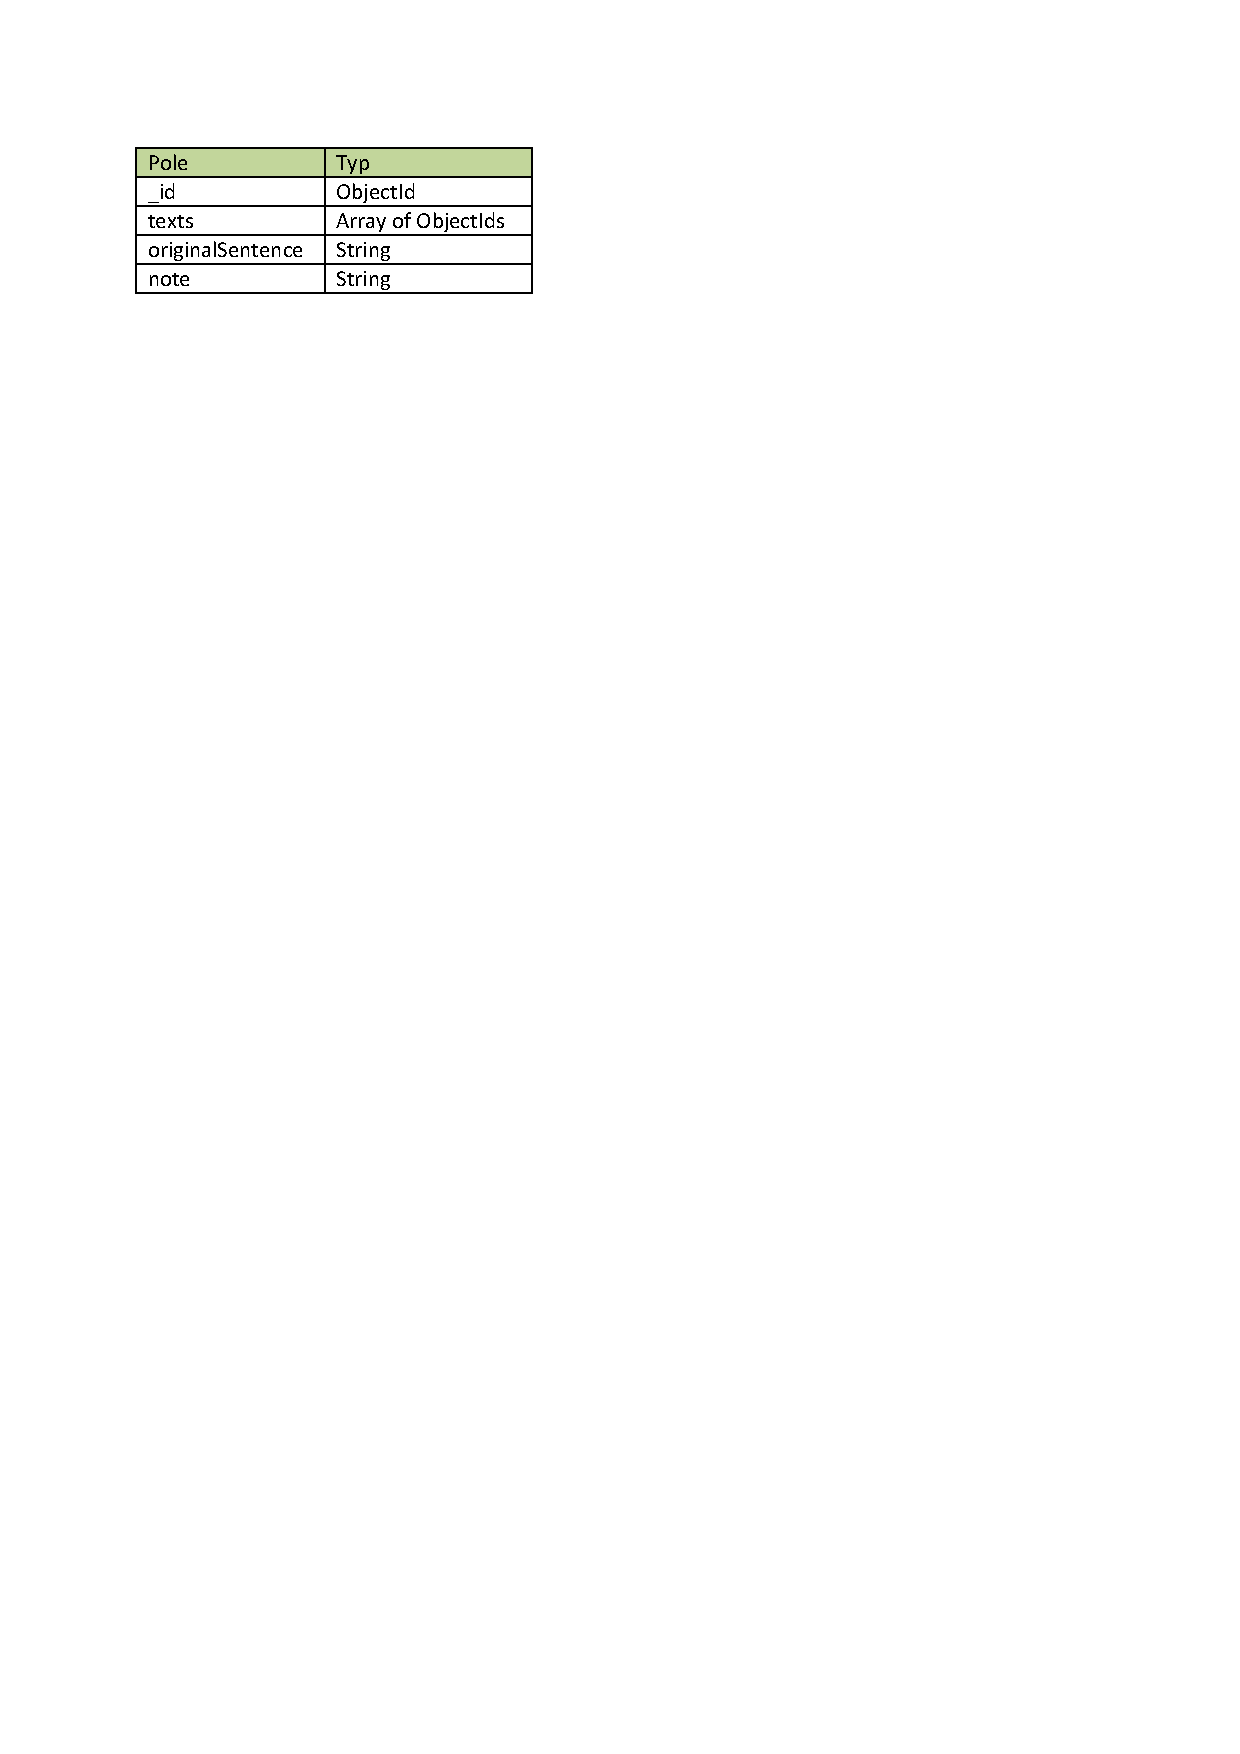
\includegraphics[scale=0.60]{sentences_collection}\end{center}
	\caption[Štruktúra kolekcie sentences]{Štruktúra kolekcie sentences}\label{fig:sentences_collection_structure}
\end{figure}

%
% Kolekcia rules
%
\ifthenelse {\boolean{bachelor}}
{
	%\subsection{Subsection}
	\subsubsection{Kolekcia rules}
}
{
	%\section{Subsection}
	\subsection{Kolekcia rules}
}
V poslednej kolekcii pomenovanej \textit{rules} sa ukladajú pravidla na spracovávanie viet, ktoré sa odkazujú na vety v kolekcii \textit{sentences}, ktoré boli podľa daného pravidla spracované. Ukladaním viet a pravidiel na ich spracovanie do separátnych kolekcií zabránime duplikovaniu dát a zrýchlime vyhľadávanie. Referencia do kolekcie \textit{sentences} nám poskytuje možnosť jednoduchého a rýchleho vyhľadanie viet, na ktoré bolo konkrétne pravidlo aplikované a aký bol výstup aplikovania tohto pravidla.

Pravidlo sa skladá hlavne z dvoch častí. Zoznam závislostí pôvodnej vety a zoznam závislostí zjednodušenej vety. Práve závislosti z druhého menovaného zoznamu sa aplikujú na spracovávanú vetu s cieľom zjednodušiť ju.

Každý záznam v tejto kolekcii obsahuje pole celých čísel určujúcich pozície slov, za ktorými je vo vytvorenej zjednodušenej vete ukončenie vety. V prípade jednoduchých viet to bude posledné slovo vety, ale pri súvetiach to môže byť viacero slov na ľubovolných miestach vety. Pre jednoduchú vetu \textit{,,The president of the Czech Republic is Miloš Zeman.''} bude toto pole obsahovať hodnotu 3, keďže zjednodušená veta bude v tvare \textit{,,President is Zeman.''}. Pre zloženú vetu v tvare \textit{,,Czech Republic has no sea; its neighbour countries are Germany, Austria, Slovakia and Poland.''} bude spomínané pole obsahovať dve hodnoty, keďže táto veta sa skladá z dvoch. Prvá obsahujúca informáciu o mori a druhá s informáciou o susedných štátoch, a tak sa aj spracuje pri zjednodušovaní.

Okrem poľa určujúceho konce viet, bude každý záznam obsahovať dva hlavné zoznamy závislostí. Prvý zoznam bude pozostávať zo závislostí pôvodnej vety a druhý zoznam bude zložený zo závislostí zjednodušenej vety. Zoznamy majú nasledujúcu štruktúru. Tieto dokumenty majú názov vzťahu závislosti a ich zoznam, pričom sa párujú práve podľa názvu. Tento vnorený zoznam obsahuje už konkrétne závislosti. Každá závislosť uložená v databáze sa skladá z nadradeného tokenu (angl. governor), podradeného tokenu (angl. dependent) a pozície tejto závislosti medzi všetkými závislosťami vety. Tokeny sú dokumenty skladajúce sa z dvoch polí, jedno textové, obsahujúce skratku POS značky a druhé číselne, obsahujúce pozíciu slova vo vete, ku ktorému sa daný token viaže.

Celá štruktúra dát v kolekcii \textit{rules} sa dá vyjadriť diagramom~\fullref{fig:rules_collection_structure}.

\begin{figure}[H]
	\begin{center}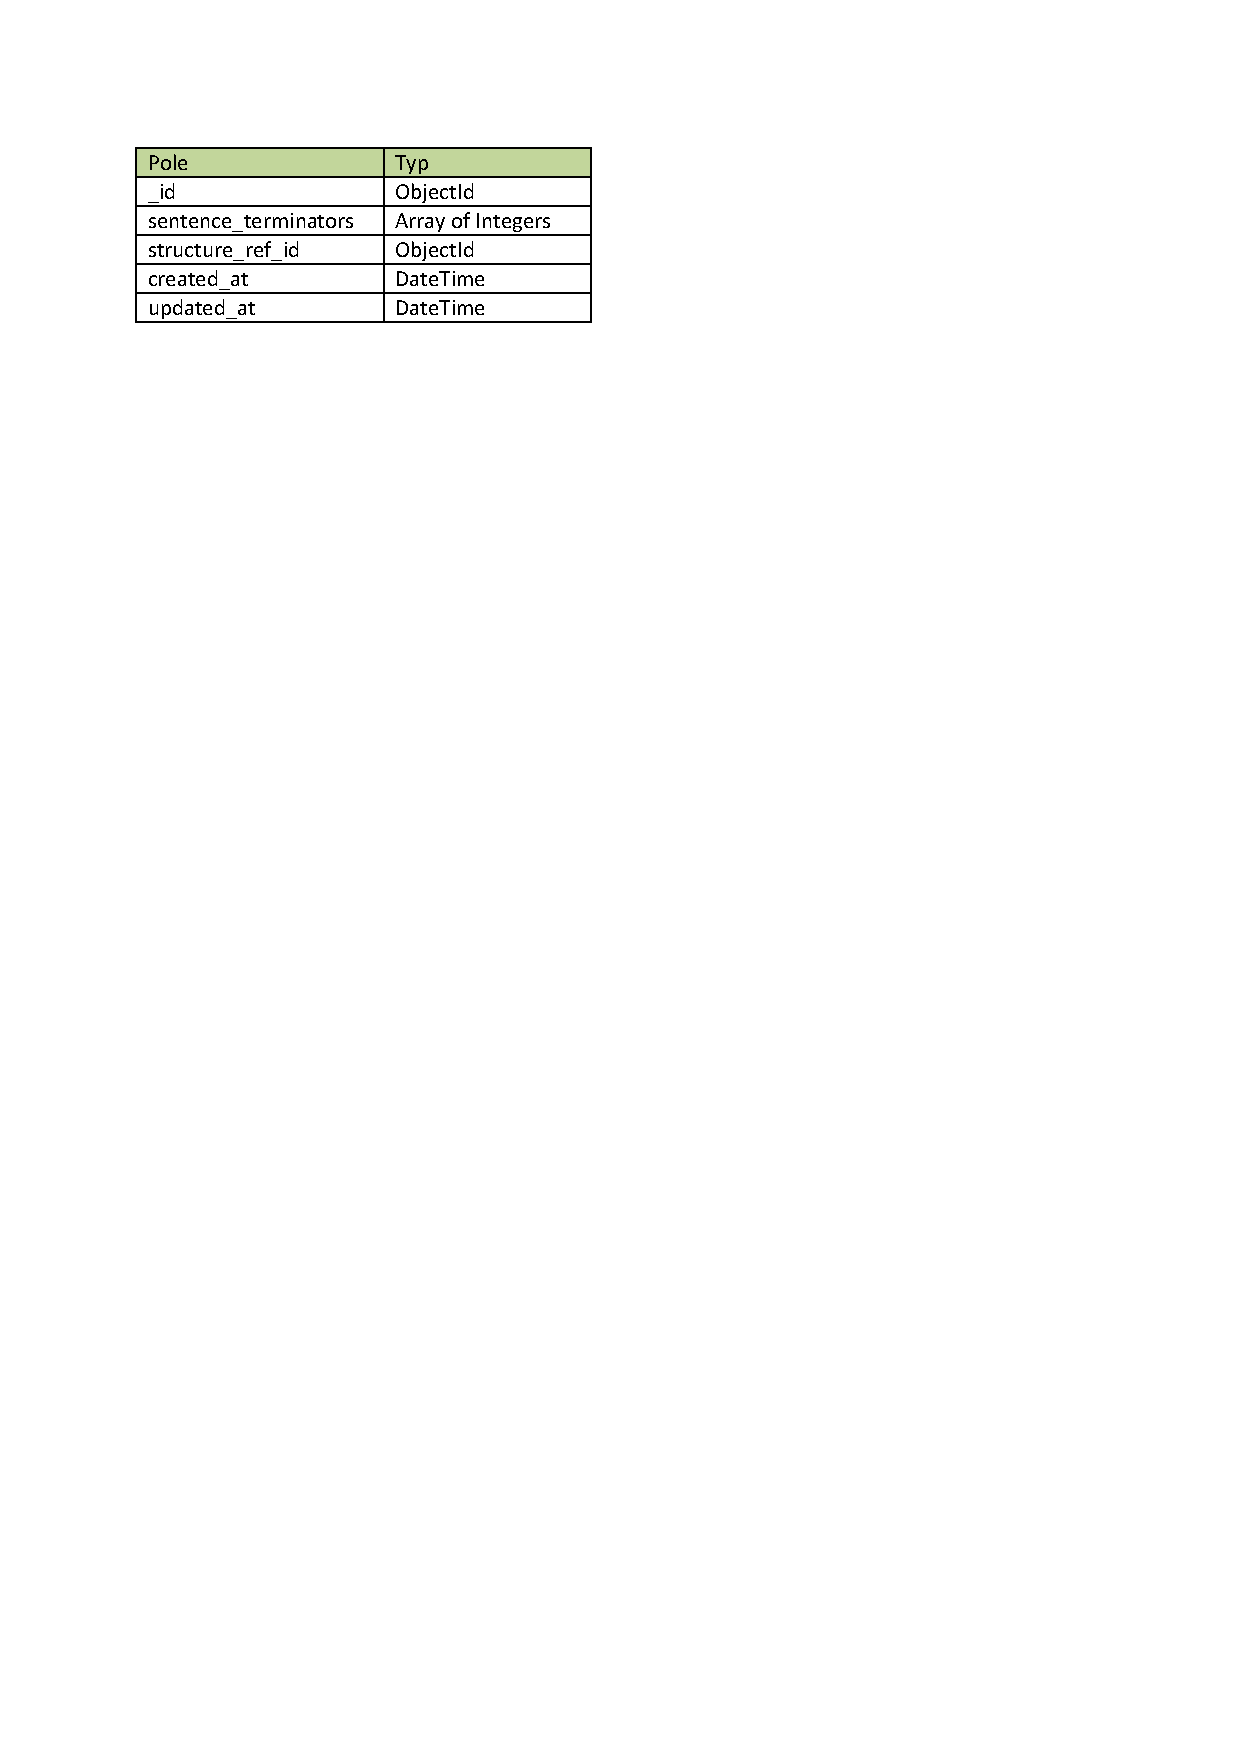
\includegraphics[scale=0.45]{rules_collection}\end{center}
	\caption[Štruktúra kolekcie rules]{Štruktúra kolekcie rules}\label{fig:rules_collection_structure}
\end{figure}

Dáta sú v MongoDB databáze uložené v binárnom JSON formáte. Na ukážke~\fullref{code:collection_rules_data_example} je zobrazená časť uložených údajov o pôvodnej vete. Ukážka celého záznamu pre vetu ,,The president of the Czech Republic is Milos Zeman.'' je priložená v prílohe~\fullref{appendix:db_entry_full_example}.
\\
\begin{lstlisting}[language = json, caption={Ukážka dát kolekcie rules}, label = {code:collection_rules_data_example}]
{  
	"originalDependencies" : [  
		{  
			"dependencyName" : "det",
			"dependencies" : [  
				{  
					"governor" : {  
						"pos" : "NN",
						"index" : 2
					},
					"dependent" : {  
						"pos" : "DT",
						"index" : 1
					},
					"position" : 0
				},
				{ ... }
			]
		}
	]
}
\end{lstlisting}


%
% Manažment dát
%
\ifthenelse {\boolean{bachelor}}
{
	%\subsection{Subsection}
	\subsection{Manažment dát}
}
{
	%\section{Subsection}
	\section{Manažment dát}
}
\label{subsection:data_management}
V nasledujúcich častiach si priblížime prácu s dátami z databázy, ako vyhľadanie pravidla, jeho aplikovanie alebo vytvorenie pravidla, ak žiadne nebolo vyhľadané.

%
% Vyhľadávanie pravidla
%
\ifthenelse {\boolean{bachelor}}
{
	%\subsection{Subsection}
	\subsubsection{Vyhľadanie pravidla}
}
{
	%\section{Subsection}
	\subsection{Vyhľadanie pravidla}
}

\label{subsubsection:rule_lookup}
Pri spracovávaní vety, pred vytvorením poznámky, aplikovateľné pravidlo musí byť vyhľadané v databáze. Závislosti pravidla a závislostí vety musia spolu korešpondovať. Pre vyhľadanie pravidla, pravidlo aj veta musia obsahovať rovnakú množinu závislostí. To znamená mať rovnaký počet záznamov v \textit{zozname dát o pôvodnej vete} a zároveň tieto záznamy musia obsahovať rovnaké názvy vzťahov závislostí.

Aplikovateľné pravidlo je vyhľadané ak hlavná podmienka je splnená. Avšak, táto podmienka môže spôsobiť, že viacero aplikovateľných pravidiel je vyhľadaných. V takom prípade zhoda spracovávanej vety a originálnej vety obdržanej z pravidla musí byť vypočítaná. Pravidlo s najväčšou zhodou je následne aplikované.

Výpočet zhody pozostáva z niekoľkých krokov. Najskôr je separátne vypočítaná zhoda POS značiek podradeného a nadradeného tokenu. Indexy nadradeného a podradeného tokenu su taktiež vypočítané separátne. Tieto prvé kroky určia, či veta obsahuje ľubovolnú závislosť s rovnakou POS značkou alebo indexom. V nasledujúcom kroku je určená polovičná zhoda závislostí. Polovičná zhoda závislosti je zhoda POS značky a indexu nadradeného alebo podradeného tokenu. Zhodu POS značky a indexu nadradeného alebo podradeného tokenu počítame pre každú závislosť. Nakoniec, v poslednom kroku, počítame počet úplne zhodných závislostí. Úplní zhoda závislosti je zhoda POS značky a indexu nadradeného, a zároveň podradeného tokenu. Každý krok ma priradené ohodnotenie. Ak je podmienka v kroku vyhodnotená ako správna, ohodnotenie kroku je pripočítané do finálnej hodnoty. Finálna zhoda je percentuálne ohodnotenie zhody. Ohodnotenie krokov odzrkadľuje dôležitosť daného kroku vo výpočte presnej zhody, pričom závisí od počtu závislostí a krokov, takže finálna zhoda nemôže presiahnuť hodnotu 100\%. Pseudokód~\ref{alg:calculating_match} zobrazuje algoritmus výpočtu zhody, konkrétny príklad je zobrazený na obrázku~\fullref{fig:calculate_match_sentences_example}

\begin{algorithm}[H]
	\floatname{algorithm}{Algoritmus}
	\footnotesize %\small, \footnotesize, \scriptsize, or \tiny
	\begin{algorithmic}[1]

		\Procedure{CalculateMatch}{$sentence, originalDependencies$}
		\State $oneCompareTypeRating \gets \text{calculate percentage rating of one comparison}$
		
		\ForAll {$originalDependencies$}
		\If {$\text{count(}sentence\text{, }dependency\text{) =  count(}originalDependencies\text{, }dependency\text{)}$}
		\State $match \gets match \text{ + } oneCompareTypeRating$
		\EndIf
		\State $counter \gets counter \text{ + } \text{count(}originalDependencies\text{, } dependency\text{)}$
		\EndFor
		
		\State $oneCompareTypeRating \gets oneCompareType / counter$
		\ForAll {$originalDependency$}
		\ForAll {$dependency$}
		\ForAll {$comparison$}
		\If {$\text{applyComparison(}sentence, comparison, dependency\text{)}$}
		\State $match \gets match \text{ + } oneCompareTypeRating$
		\EndIf
		\EndFor
		\EndFor
		\EndFor
		
		\Return $match$
		\EndProcedure
	\end{algorithmic}
	\caption[Výpočet zhody]{Výpočet zhody}	
	\label{alg:calculating_match}
\end{algorithm}

\begin{figure}[H]
	\begin{center}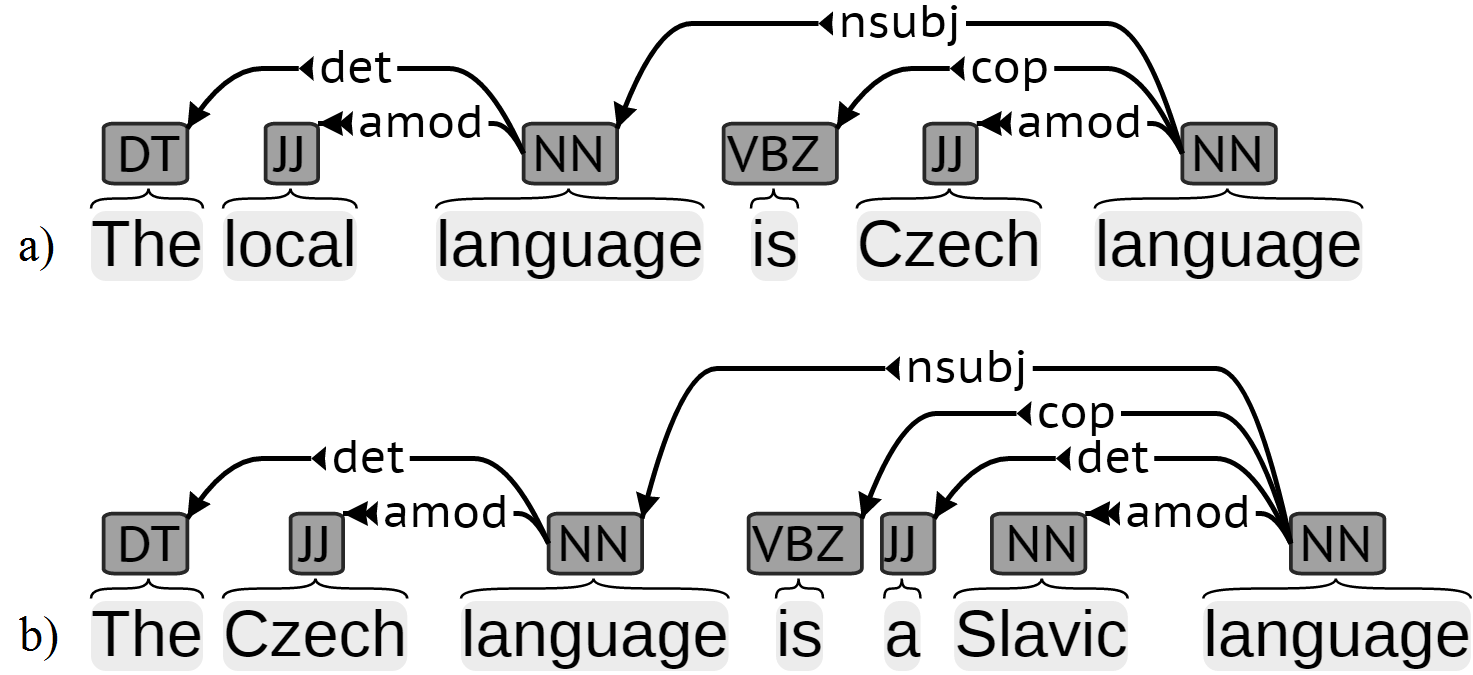
\includegraphics[scale=0.2]{calculate_match_sentences_example}\end{center}
	\caption[Príklad určenia zhody]{Príklad určenia zhody}\label{fig:calculate_match_sentences_example}
\end{figure}

Predpokladajme situáciu z obrázka~\fullref{fig:calculate_match_sentences_example}. Máme pravidlá pre dve vety s spracovávame prvú z nich. V tejto situácií, minimálne dve pravidlá su aplikovateľné na vetu \textit{a}. Predpokladajme, že vypočítavame zhodu s vetou \textit{b}. Prechádzame postupne cez všetky závislosti spracovávanej vety \textit{a}. Prvá závislosť je so vzťahom \textit{det}, nadradeným tokenom s POS značkou NN (noun - podstatné meno) a indexom 3 a podradeným tokenom s POS značkou DT (determiner - determinant) a indexom 1. V prvok kroku zistíme, či veta \textit{b} obsahuje závislosť so vzťahom \textit{det} a tokenmi s POS značkami NN alebo DT and indexmi rovnými 1 alebo 3. Toto je separátny výpočet POS značiek a indexov. v nasledujúcom kroku zisťujeme, či veta \textit{b} obsahuje závislosť so vzťahom \textit{det} a nadradeným alebo podradeným tokenom s POS značkou NN a indexom 3 alebo POS značkou DT a indexom 1. Toto je polovičná zhoda. V poslednom kroku hľadáme vo vete \textit{b} závislosť so vzťahom \textit{det} a nadradeným tokenom práve s POS značkou NN a indexom 3 a zároveň podradený token práve s POS značkou DT a indexom 1. Ak ktorýkoľvek krok bol vyhodnotený ako správny, jeho ohodnotenie je pridané ku koncovému výsledku a iterácia pokračuje s nasledujúcou závislosťou, pokým sa nevyhodnotí posledná.

Aplikovaním určenia zhody vety \textit{a} s vetami \textit{a} a \textit{b} zistíme, že s vetou \textit{a} má zhodu $100\%$ a s vetou \textit{b} má cca. $63,57\%$ zhodu.

%\begin{figure}[H]
%	\begin{center}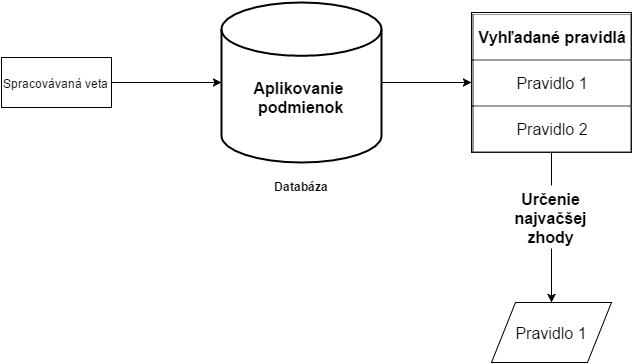
\includegraphics[scale=0.6]{rule_lookup}\end{center}
%	\caption[Vyhľadanie pravidla]{Vyhľadanie pravidla}\label{fig:rule_lookup}
%\end{figure}

%
% Aplikovanie pravidla
%
\ifthenelse {\boolean{bachelor}}
{
	%\subsection{Subsection}
	\subsubsection{Aplikovanie pravidla}
}
{
	%\section{Subsection}
	\subsection{Aplikovanie pravidla}
}
\label{subsubsection:rule_application}

Z princípu vyhľadania pravidla (viď.~\fullref{subsubsection:rule_lookup}), spracovávaná veta musí obsahovať, nie všetky, závislostí zo \textit{zoznamu dát pôvodnej vety}, vety prepojenej s pravidlom a tým pádom aj závislostí zo \textit{zoznamu dát poznámky} pravidla.

Proces aplikovania pravidla na vetu s cieľom vytvorenia poznámky sa skladá z niekoľkých krokov. Pre všetky závislosti zo \textit{zoznamu dát poznámky}, príslušná závislosť je vyhľadaná v spracovávanej vete. Pri vyhľadávaní príslušnej závislosti sa závislosti neporovnávajú, okrem iného, na základe POS značiek svojich tokenov, ale podľa nadradených POS značiek svojich tokenov. To znamená, že ak token obsahuje POS značku NNP (proper noun, singular - [SLOVENSKY EKVIVALENT]), jeho nadradaná POS značka je NN (noun - podstatné meno). Vyhľadáva sa teda podľa množiny POS značiek podstatného mena, a to konkrétne \textit{NN, NNS, NNP} a \textit{NNPS}. Tento spôsob vyhľadávania nám umožňuje [BLA BLA, blizie opisane v BLA BLA]. Avšak, môže to spôsobiť vyhľadanie viac ako jednej príslušnej závislosti. Preto zhoda závislostí musí byť vypočítaná (viď.~\nameref{paragraph:dependency_match} na strane \pageref{paragraph:dependency_match}). Po vypočítaní zhody závislosti a získanie závislosti s najväčšou zhodou, slovo korešpondujúce s tokenom, ktorý sa ma z danej závislosti vybrať, sa pridá do poznámky na pozíciu indexu tokenu. Po spracovaní všetkých závislostí, posledné minoritné úpravy su vykonané nad poznámkou, ako napríklad rozdelenie na viacero viet, ak tak určovalo pravidlo, kapitalizácia prvých písmen viet poznámky a iné. Pseudokód aplikovania pravidla na vetu s cieľom vytvoriť poznámku je zobrazený na algoritme~\ref{alg:applying_rule}.

\begin{algorithm}
	\floatname{algorithm}{Algoritmus}
	\caption[Aplikovanie pravidla]{Aplikovanie pravidla}\label{alg:applying_rule}
	\begin{algorithmic}[1]
		\Procedure{ApplyRule}{$sentence, rule$}
		\State $note \gets \text{new Note}$
		\ForAll {$ruleDependencies$}
		\State $dependency \gets \text{findDependency(} sentence \text{, } ruleDependency \text{)}$
		\If {$\text{isFound(}dependency\text{)}$}
		\State $\text{add(} note \text{, getDependent(} dependency \text{))}$
		\If {$\text{isNominalSubject(relation(}dependency \text{))}$}
		\State $\text{add(} note \text{, getGovernor(} dependency \text{))}$
		\EndIf
		\EndIf
		\EndFor
		
		\State $\text{splitToSentences(} note \text{, sentencesEnds(} rule \text{))}$	
		
		\Return $note$
		\EndProcedure
	\end{algorithmic}
\end{algorithm}

Pre vetu ,,The president of the Slovak republic is Andrej Kiska.'' nám nástroj Stanford CoreNLP poskytne závislostí vyobrazené na obrázku~\fullref{fig:example_sentence_andrej_kiska}. Ak na túto vetu aplikujeme pravidlo v tvare zobrazené na obrázku~\fullref{fig:apply_rule_example_rule}, výsledná poznámka bude ,,President is Kiska.''. 

\begin{figure}[H]
	\begin{center}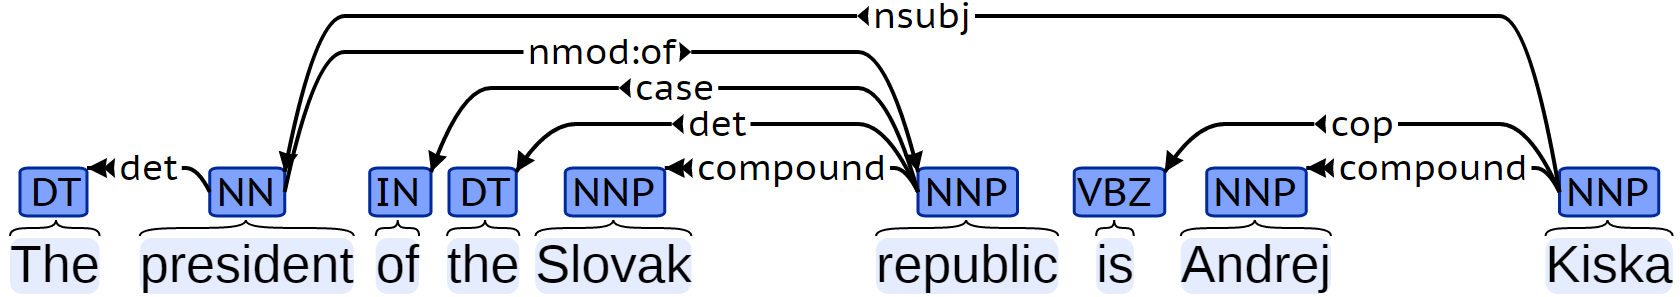
\includegraphics[scale=0.32]{example_sentence_andrej_kiska}\end{center}
	\caption[Zásivlostí jednoduchej vety]{Zásivlostí jednoduchej vety}\label{fig:example_sentence_andrej_kiska}
\end{figure}

\begin{figure}[H]
	\begin{center}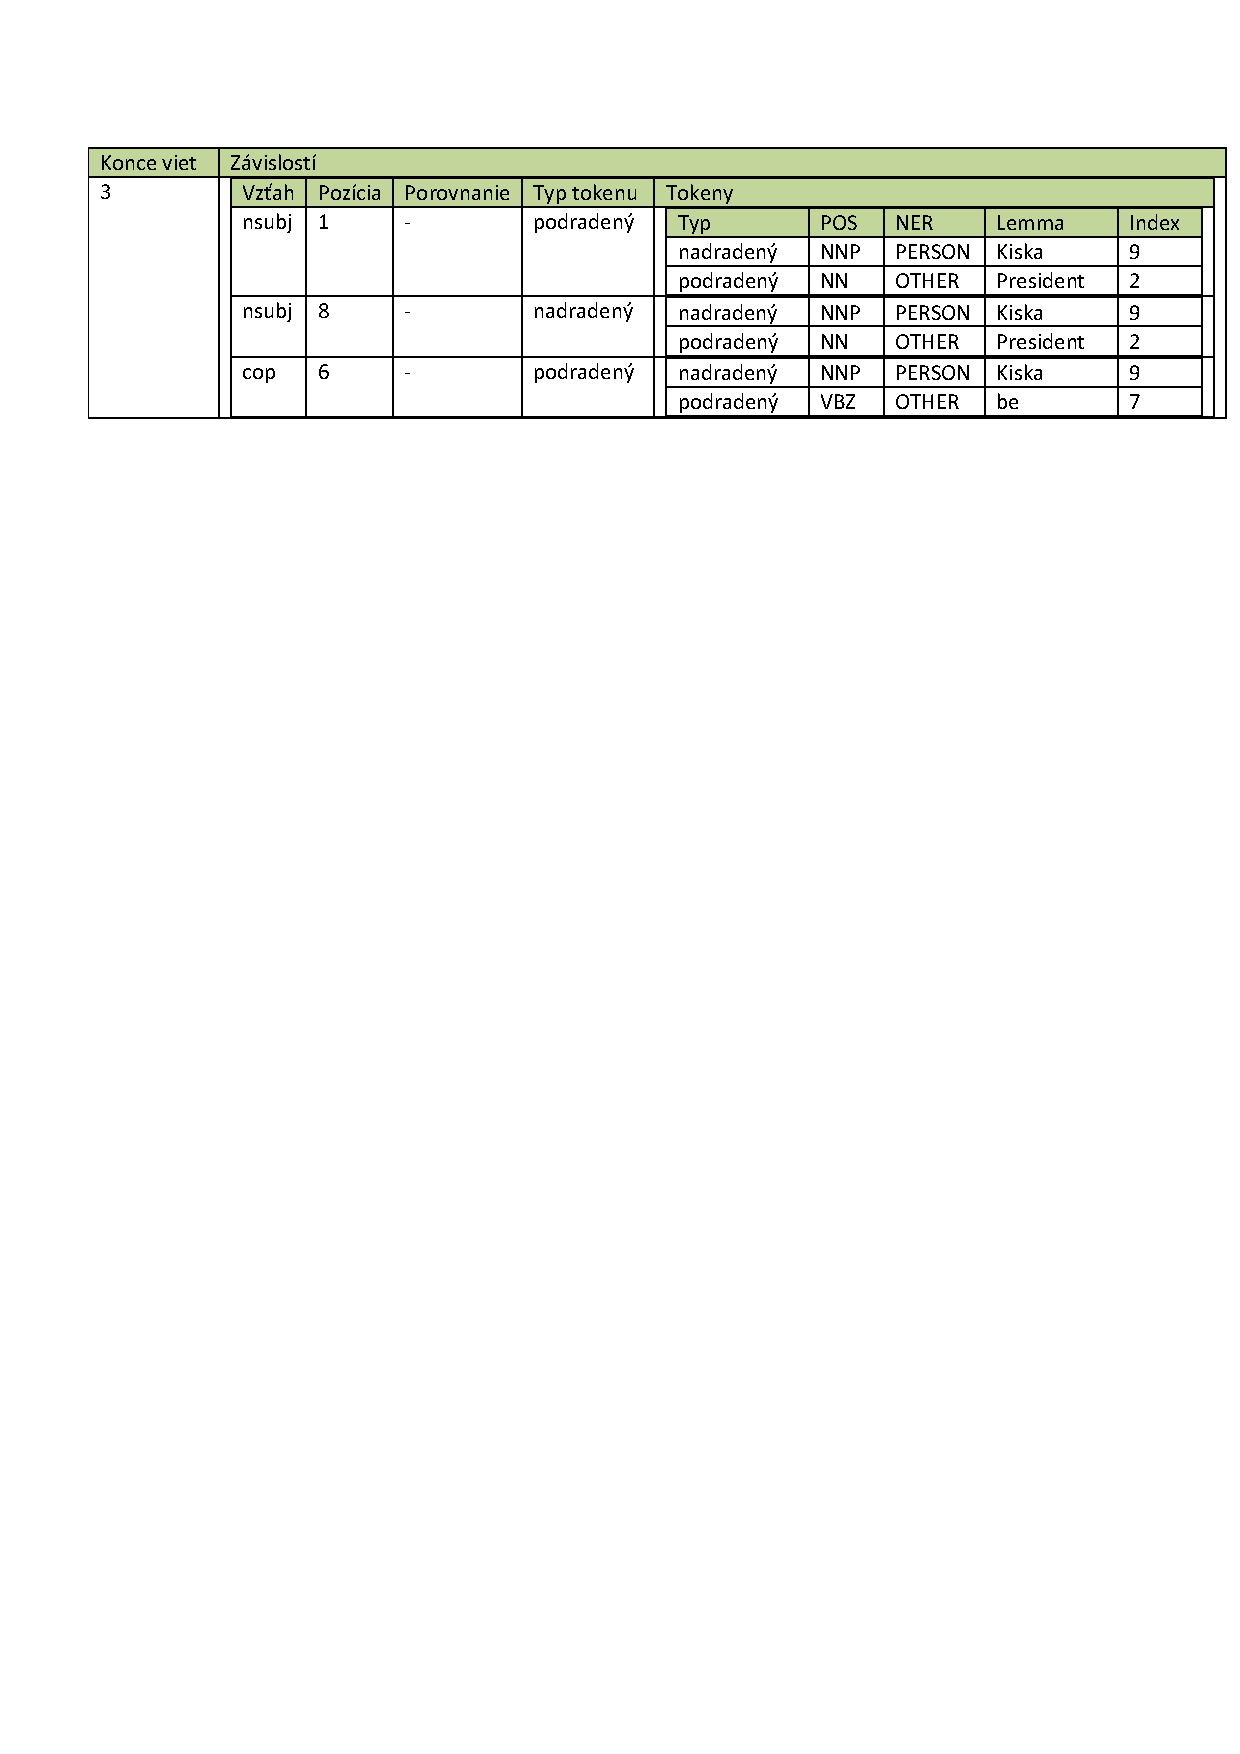
\includegraphics[scale=0.32]{apply_rule_example_rule}\end{center}
	\caption[Príklad pravidla]{Príklad pravidla}\label{fig:apply_rule_example_rule}
\end{figure}

%
% Výpočet zhody závislostí
%
\ifthenelse {\boolean{bachelor}}
{
	%\subsection{Subsection}
	\paragraph{Výpočet zhody závislostí}
}
{
	%\section{Subsection}
	\subsubsection{Výpočet zhody závislostí}
}
\label{paragraph:dependency_match}

Výpočet zhody závislostí pozostáva s niekoľkých krokov a princíp výpočtu je veľmi podobný s výpočtom zhody viet zo sekcie~\fullref{subsubsection:rule_lookup}. Porovnávajú sa vždy nadradené aj podradené tokeny. Porovnanie ma niekoľko krokov. Začína sa s porovnaním POS značiek. Pokračuje sa názvoslovnou entitou, indexom, lemou a nakoniec sa porovná vzdialenosť pozícií tokenov vo vetách. Každý krok je príslušne ohodnotený a ak porovnanie bolo úspešné, ohodnotenie sa pripočíta k finálnej hodnote reprezentujúca percentuálne zhodu závislostí.

%
% Vytváranie pravidla
%
\ifthenelse {\boolean{bachelor}}
{
	%\subsection{Subsection}
	\subsubsection{Vytvorenie pravidla}
}
{
	%\section{Subsection}
	\subsection{Vytvorenie pravidla}
}
\label{subsubsection:rule_creation}
Ak nám proces vyhľadania pravidla nevyhľadal žiadne pravidlo, znamená to, že sme doposiaľ nespracovávali takú istú alebo podobnú vetu. V tomto prípade sú použité statické pravidlá na spracovanie vety. Výstupom bude zjednodušená veta - poznámka.

Vytvorí sa záznam o pôvodnej vete, ktorý okrem iného obsahuje \textit{zoznam dát o pôvodnej vete}, ktorý sa vyskladá zo závislostí vety. Následne sa vytvorí záznam o pravidle, ktorý okrem iného obsahuje \textit{zoznam dát o poznámke}, vyskladaný zo závislosti poznámky. Nakoniec sa tieto dva záznamy prepoja a tým sa vytvorí nové pravidlo na spracovanie takej istej alebo podobnej vety, akú sme práve spracovali.

Na obrázku~\fullref{fig:rule_creation} je znázornený proces nevyhľadania pravidla, použitia parsera s následným uložením nového pravidla.

\begin{figure}[H]
	\begin{center}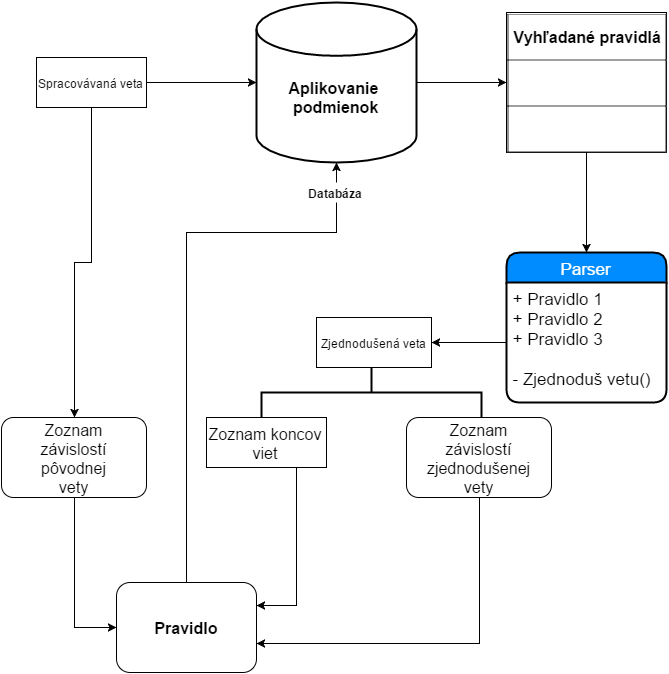
\includegraphics[scale=0.5]{rule_creation}\end{center}
	\caption[Vytvorenie pravidla]{Vytvorenie pravidla}\label{fig:rule_creation}
\end{figure}